\documentclass[nobib]{tufte-handout}

\newcommand{\bra}[1]{\left(#1\right)}
\usepackage{amssymb}
\usepackage{hyperref}
\usepackage{pgfplots}
\usepackage[activate={true,nocompatibility},final,tracking=true,kerning=true,spacing=true,factor=1100,stretch=10,shrink=10]{microtype}
\usepackage{color}
\usepackage{steinmetz}
\usepackage{placeins}
\usepackage{marginfix}
\usepackage{array}
\usepackage{tikz}
\usepackage{amsmath,amsthm}
\usetikzlibrary{shapes, arrows, positioning, calc}
\tikzset{block/.style={draw, rectangle, minimum height=1.5em, minimum width=3em},
         sum/.style={draw, circle, inner sep=0pt, minimum size=2mm},
         >=latex'}
\usepackage{listings}
\usepackage{forest}
\usepackage{caption}
\DeclareCaptionFont{white}{\color{white}}
\DeclareCaptionFormat{listing}{\colorbox{gray}{\parbox{\textwidth}{#1#2#3}}}
\captionsetup[lstlisting]{format=listing,labelfont=white,textfont=white}
\usepackage{graphicx}
\setkeys{Gin}{width=\linewidth,totalheight=\textheight,keepaspectratio}
\graphicspath{{.}}

\title{ECE 30200 - Probabilistic Methods in Electrical and Computer Engineering}
\author{Zeke Ulrich}
\date{\today}  % if the \date{} command is left out, the current date will be used

\usepackage{booktabs}
\usepackage{units}
\usepackage{fancyvrb}
\fvset{fontsize=\normalsize}
\usepackage{multicol}

\begin{document}

\maketitle

\tableofcontents

\pagebreak

\section{Background}

The following formulas will be instrumental and may be familar.

\subsection{Series}
\begin{equation}
    \sum_{k=0}^{n} r^k = \frac{1 - r^{n + 1}}{1 - r}
\end{equation}
\begin{equation}
    \sum_{n=1}^{\infty} \frac{1}{n^2} = \frac{\pi^2}{6}
\end{equation}
\begin{equation}
    \sum_{k=1}^{\infty}kr^{k - 1} = \frac{1}{(1 - r)^2}
\end{equation}

\subsection{Combinatorics}
\begin{equation}
    {n\choose k} = \frac{n!}{k!(n - k)!}
\end{equation}
\begin{equation}
    (a + b)^n = \sum_{k=0}^{n} {n\choose k} a^{n - k}b^k
\end{equation}
\begin{equation}
    {n\choose k} + {n\choose k-1} = {n + 1\choose k}
\end{equation}
\begin{equation}
    P(n, k) = \frac{n!}{(n-k)!}
\end{equation}
where $P(n, k)$ is the number of ways to arrange $k$ objects out of $n$ (permutations).
\begin{equation}
    C(n, k) = {n\choose k} = \frac{n!}{k!(n-k)!}
\end{equation}
where $C(n, k)$ is the number of ways to choose $k$ objects out of $n$ (combinations).

\subsection{Approximations}
\begin{align}
    f(x) & = f(a) + f'(a)(x - a) + \frac{f''(a)}{2!}(x - a)^2 + \dots \\
         & = \sum_{n=0}^{\infty} \frac{f^{(n)}(a)}{n!}(x - a)^n
\end{align}
\begin{align}
    1 + x + \frac{x^2}{2!} + \frac{x^3}{3!} + \dots & = \sum_{k=0}^{\infty} \frac{x^k}{k!} \\
                                                    & = e^x
\end{align}
\begin{align}
    \sin(x) & = x - \frac{x^3}{3!} + \frac{x^5}{5!} - \frac{x^7}{7!} + \dots \\
            & = \sum_{n=0}^{\infty} (-1)^n \frac{x^{2n+1}}{(2n+1)!}
\end{align}
\begin{align}
    \cos(x) & = 1 - \frac{x^2}{2!} + \frac{x^4}{4!} - \frac{x^6}{6!} + \dots \\
            & = \sum_{n=0}^{\infty} (-1)^n \frac{x^{2n}}{(2n)!}
\end{align}
\begin{align}
    \ln(1 + x) & = x - \frac{x^2}{2} + \frac{x^3}{3} - \frac{x^4}{4} + \dots \\
               & = \sum_{n=1}^{\infty} (-1)^{n+1} \frac{x^n}{n}
\end{align}

\subsection{Calculus}
\begin{equation}
    \frac{d}{dx} \int_{a}^{x} f(t)\,dt = f(x)
\end{equation}
\begin{equation}
    \int_{a}^{b} f'(x)\,dx = f(b) - f(a)
\end{equation}
\begin{equation}
    \int f(g(x))g'(x)\,dx = \int f(u)\,du
\end{equation}
\begin{equation}
    \int u\,dv = uv - \int v\,du
\end{equation}
\begin{equation}
    \int \frac{1}{(x-a)(x-b)}\,dx = \frac{1}{b-a} \ln\left|\frac{x-a}{x-b}\right| + C
\end{equation}

\subsection{Linear Algebra}
\begin{equation}
    \vec{y} = \beta_1 \vec{x_1} + \beta_2 \vec{x_2} + \cdots + \beta_N \vec{x_N}
\end{equation}
\begin{align}
    \langle \vec{a}, \vec{b} \rangle & = \vec{a}\vec{b}^{T}     \\
                                     & = \sum_{i=1}^{n} a_i b_i
\end{align}
where $\langle \vec{a}, \vec{b} \rangle$ denotes the inner product of vectors $\vec{a}$ and $\vec{b}$.
\begin{equation}
    \|\vec{x}\|_p = \left( \sum_{i=1}^{n} |x_i|^p \right)^{1/p}
\end{equation}
where $\|\vec{x}\|_p$ is the $p$-norm (or $\ell_p$-norm) of vector $\vec{x}$.
\begin{equation}
    \cos(\theta) = \frac{\langle \vec{a}, \vec{b} \rangle}{\|\vec{a}\|_2 \|\vec{b}\|_2}
\end{equation}
where $\theta$ is the angle between vectors $\vec{a}$ and $\vec{b}$.
\begin{equation}
    \hat{\beta} = (\mathbf{X}^T \mathbf{X})^{-1} \mathbf{X}^T \vec{y}
\end{equation}
where $\hat{\beta}$ is the vector of least squares coefficients, $\mathbf{X}$ is the data matrix, and $\vec{y}$ is the target vector

\subsection{Set Theory}
Some important properties of set operations are:
\begin{itemize}
    \item \textbf{Commutativity:}
          \begin{align}
              A \cup B & = B \cup A \\
              A \cap B & = B \cap A
          \end{align}
    \item \textbf{Associativity:}
          \begin{align}
              (A \cup B) \cup C & = A \cup (B \cup C) \\
              (A \cap B) \cap C & = A \cap (B \cap C)
          \end{align}
    \item \textbf{Distributivity:}
          \begin{align}
              A \cup (B \cap C) & = (A \cup B) \cap (A \cup C) \\
              A \cap (B \cup C) & = (A \cap B) \cup (A \cap C)
          \end{align}
    \item \textbf{Identity:}
          \begin{align}
              A \cup \emptyset & = A \\
              A \cap \Omega    & = A
          \end{align}
    \item \textbf{Complement:}
          \begin{align}
              A \cup A^c & = \Omega    \\
              A \cap A^c & = \emptyset
          \end{align}
\end{itemize}

\subsection{Probability Laws}
A probability law must satisfy three axioms:
\begin{enumerate}
    \item Non-negativity: $P(A) \geq 0 \forall A \in F$
    \item Normalization: $P(\Omega) = 1$
    \item Additivity: For any disjoint subsets $\{A_1, A_2, \dots\}$,
          it holds that
          \[P\left[\bigcup_{n=1}^{\infty}A_n\right] = \sum_{n=1}^{\infty}P\left[A_n\right]\]
\end{enumerate}

\subsection{Probability Properties}
\begin{equation}
    P\left[A \cup B\right] = P\left[A\right] + P\left[B\right] - P\left[A \cap B\right]
\end{equation}
\begin{equation}
    P\left[A \cup B\right] \leq P\left[A\right] + P\left[B\right]
\end{equation}
\begin{equation}
    A \subseteq B \implies P\left[A\right] \leq P\left[B\right]
\end{equation}
\section{Formal Definitions}

\subsection{Outcomes}
An \emph{outcome} is the result of some \emph{experiment}.
If that experiment is flipping a coin, the outcome is either
heads or tails. We could express the outcome of heads as $H$,
and the outcome of tails as $T$. The set of all possible
outcomes for an experiment is known as a sample space and is
denoted by $\Omega$. In this case $\Omega = \{H, T\}$.

\subsection{Events}
An \emph{event} $F$ is a subset of the sample space $\Omega$.
The formal definitions of probability are expressed with set
notation. So the event where we have neither heads nor tails is
written as $\{\}$. The event of heads could be expressed as
$\{H\}$, and the event of tails could be expressed as $\{T\}$.
The event of either heads or tails is $\{H, T\}$.

\subsection{Probability Laws}
A \emph{probability law} is a function $P$ that maps an event $A$
to a real number in $[0, 1]$. For the coin example, the probability
law might be $P(\{\}) = 0$, $P(\{H\}) = 0.5$, $P(\{T\}) = 0.5$, and
$P(\{\Omega\}) = 1$. A probability law must satisfy three axioms:
\begin{enumerate}
    \item Non-negativity: $P(A) \geq 0 \forall A \in F$
    \item Normalization: $P(\Omega) = 1$
    \item Additivity: For any disjoint subsets $\{A_1, A_2, \dots\}$,
          it holds that
          \[P\left[\bigcup_{n=1}^{\infty}A_n\right] = \sum_{n=1}^{\infty}P\left[A_n\right]\]
\end{enumerate}

\subsection{Probability Space}
A probability space is a triplet $\Omega, F, P$.

\subsection{Probability Properties}
\begin{equation}
    P\left[A \cup B\right] = P\left[A\right] + P\left[B\right] - P\left[A \cap B\right]
\end{equation}
\begin{equation}
    P\left[A \cup B\right] \leq P\left[A\right] + P\left[B\right]
\end{equation}
\begin{equation}
    A \subseteq B \implies P\left[A\right] \leq P\left[B\right]
\end{equation}
\begin{equation}
    P\left[A | B\right] = \frac{P[A \cap B]}{P[B]}
\end{equation}

Outcomes are statistically \emph{independent} if
$P(A|B) = P(A)$ (assuming P(B) > 0), or
equivalently $P(A \cap B) = P(A)P(B)$.

A \emph{random variable} $X$ is a function $X : \Omega \implies \Re$
that maps an outcome $\epsilon \in \Omega$ to a number $X(\epsilon)$ on the real line.
We call it a variable because it has multiple states. The mapping $X$

\emph{Bayes Theorem} states that for any two events $A$ and $B$ such that $P[A] > 0$ and
$P[B] > 0$,
\begin{equation}
    P[A|B] = \frac{P[B|A]P[A]}{P[B]}
\end{equation}

The \emph{Law of Total Probability} states that if
$\{A_1, A_2, \dots, A_n\}$ is a partition of $\Omega$,
then for any $B \subseteq \Omega$,
\begin{equation}
    P[B] = \sum_{i = 1}^{n} P[B|A_i]P[A_i]
\end{equation}
\section{Discrete Random Variables}

A \emph{random variable} $X$ is a function $X : \Omega \implies \Re$
that maps an outcome $\epsilon \in \Omega$ to a number $X(\epsilon)$ on the real line.
We call it a variable because it has multiple states.

The \emph{expectation} of a random variable $X$ is
\begin{equation}
    E[X] = \sum_{x\in X(\Omega)} xp_X(x)
\end{equation}
The difference between $E[X]$ and the mean is
that $E[X]$ is computed from the ideal histogram,
while mean is computed from the empirical histogram.
In general for any functions $g$ and $h$,
\begin{align}
    E[g(X)]        & = \sum_{x} g(x)p_X(x) \\
    E[g(X) + h(X)] & = E[g(X)] + E[h(X)]   \\
    E[cX]          & = cE[X]               \\
    E[X + c]       & = E[X] + c
\end{align}

The \emph{variance} of a random variable $X$ is
\begin{equation}
    Var[X] = E\left[(X-\mu)^2\right]
\end{equation}
or alternatively, the second moment
minus the first moment squared.
\begin{equation}
    E[X^2] - E[X]^2
\end{equation}

The \emph{probability mass function} (PMF) $p_X(a)$
of a random variable $X$ specifies the probability of
obtaining a number $X(\epsilon) = a$. We denote a PMF as
\begin{equation}
    p_X(a) = P[X = a]
\end{equation}
PMFs are represented with histograms.
\begin{figure}[h]
    \centering
    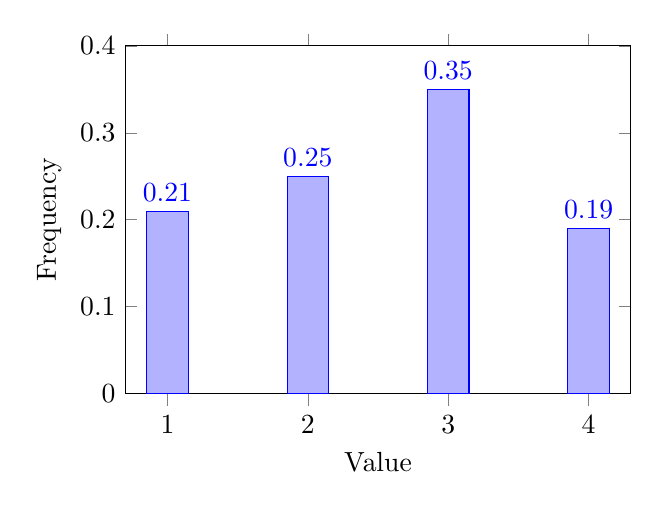
\begin{tikzpicture}
        \begin{axis}[
                ybar,
                bar width=15pt,
                xlabel={Value},
                ylabel={Frequency},
                xtick=data,
                ymin=0,
                ymax=0.4,
                nodes near coords,
                width=8cm,
                height=6cm
            ]
            \addplot coordinates {(1,0.21) (2,0.25) (3,0.35) (4,0.19)};
        \end{axis}
    \end{tikzpicture}
    \caption{PMF}
\end{figure}
A PMF should satisfy
\begin{equation}
    \sum_{x\in X(\Omega)} p_X(x) = 1
\end{equation}

The \emph{cumulative distribution function} is given by
\begin{align}
    F_X(x) & = P\left[X \leq x\right] \\
           & = \sum_{u \leq x} p_X(u)
\end{align}
and represents the sum of every impulse
of the PMF up to $x$.

A \emph{Bernoulli random variable} has a state
of either 0 or 1. The probability of getting 1 is $p$ and
the probability of getting 0 is $1 - p$. We write
\begin{equation}
    X \sim Bernoulli(p)
\end{equation}
or
\begin{equation}
    X \sim B(p)
\end{equation}
to say that $X$ is drawn from a Bernoulli distribution
with a parameter $p$. For a Bernoulli distribution,
\begin{align}
    E[X]   & = p        \\
    E[X^2] & = p        \\
    Var[X] & = p(1 - p)
\end{align}
Say $S \sim B(1-p)$.
Let
\begin{align}
    P(R=0|S=0) & = 1 - \epsilon_0 \\
    P(R=1|S=0) & = \epsilon_0
\end{align}
then $R|S=0 \sim B(\epsilon_0)$.
Let
\begin{align}
    P(R=0|S=1) & = \epsilon_1     \\
    P(R=1|S=0) & = 1 - \epsilon_1
\end{align}
then $R|S=0 \sim B(1 - \epsilon_1)$.
Overall,
\begin{equation}
    R|S \sim B(\epsilon_0^{1-S}(1-\epsilon_1)^S)
\end{equation}

A \emph{Rademacher random variable} has two states, -1 and 1.
The probability of getting each is 0.5.

A \emph{binomial random variable} has a PMF of
\begin{equation}
    p_X(k) = {n\choose k} p^k (1 - p)^{n - k}, k = 0, 1, \dots n
\end{equation}
where $0 < p < 1$ is the binomial parameter, and $n$ is the total
number of states. We write
\begin{equation}
    X \sim Binomial(n, p)
\end{equation}
to say that $X$ is drawn from a binomial distribution with a
parameter $p$ of size $n$.
If $X \sim Binomial(n, p)$, then
\begin{align}
    E[X]   & = np               \\
    E[X^2] & = np(np + (1 - p)) \\
    Var[X] & = np(1 - p)
\end{align}

Let $X$ be a \emph{geometric random variable}. Then the
PMF of $X$ is
\begin{equation}
    p_X(k) = (1 - p)^{k - 1}p, k=1,2,\dots
\end{equation}
We write
\begin{equation}
    X \sim Geometric(p)
\end{equation}
to say that $X$ was drawn from a geometric
distribution with a parameter $p$.
If $X \sim Geometric(p)$ then
\begin{align}
    E[X]   & = \frac{1}{p}                 \\
    E[X^2] & = \frac{2}{p^2} - \frac{1}{p} \\
    Var[X] & = \frac{1 - p}{p^2}
\end{align}

Let $X$ be a \emph{Poisson random variable}. Then the PMF
of $X$ is
\begin{equation}
    p_X(k) = \frac{\lambda^k}{k!}e^{-\lambda}, k=0, 1, 2,\dots
\end{equation}
where $\lambda > 0$ is the Poisson rate. We write
$X \sim Poisson(\lambda)$ to say that $X$ was drawn from
a Poisson distribution with a parameter $\lambda$.
If $X \sim Poisson(\lambda)$ then
\begin{align}
    E[X]   & = \lambda             \\
    E[X^2] & = \lambda + \lambda^2 \\
    Var[X] = \lambda
\end{align}
For small $p$ and large $n$,
\begin{equation}
    {n\choose k}p^k(1-p)^{n-k} \approx \frac{\lambda^k}{k!}e^{-\lambda}
\end{equation}

\emph{Joint Distributions} are higher-dimensional
PDFs, PMFs, or CDFs. We write
\begin{equation}
    f_{X_1, X_2, \dots, X_n}(x_1, x_2, \dots, x_n) \equiv f_{\vec{X}}(\vec{x})
\end{equation}

The \emph{joint PMF} of two random variables
$X$ and $Y$ is notated by
\begin{equation}
    p_{X,Y}(x,y)=P[X=x \text{ and } Y=y]
\end{equation}
and represents the probability of both.

A \emph{marginal PMF} is defined as
\begin{equation}
    p_X(x) = \sum_{y\in \Omega_Y} p_X(x,y)
\end{equation}
or w.l.o.g.
\begin{equation}
    p_Y(y) = \sum_{x\in \Omega_X} p_X(x,y)
\end{equation}
That is, it is the joint PMF summed over
one of the variables.

The \emph{conditional PMF} is given by
\begin{equation}
    p_{X|Y}(x|y) = \frac{p_{X,Y}(x,y)}{p_{Y}(y)}
\end{equation}

If two random variables $X$ and $Y$ are independent,
then
\begin{align}
    p_{X,Y}  & = p_X(x)p_Y(y) \\
    f_{X, Y} & = f_X(x)f_Y(y)
\end{align}
If a sequence of random variables
$X_1, X_2, \dots, X_N$ are independent,
then their joint PDF (or joint PMF) can be
factorized as
\begin{equation}
    f_{X_1,X_2,\dots,X_N}\left(x_1,x_2,\dots,x_N\right) = \prod_{n=1}^{N}f_{X_n}(x_n)
\end{equation}

The \emph{joint CDF} of two random variables
$X$ and $Y$ is the function $F_{X,Y}(x,y)$ such
that
\begin{equation}
    F_{X,Y}(x,y) = P\left[X \leq x \cap Y \leq y\right]
\end{equation}
If $X$ and $Y$ are discrete, then
\begin{equation}
    F_{X,Y}(x,y) = \sum_{y'\leq y}\sum_{x' \leq x} p_{X,Y}(x',y')
\end{equation}

For two random variables $X$ and $Y$,
the \emph{marginal CDF} is
\begin{align}
    F_X(x) & = F_{X,Y}(x, \infty) \\
    F_Y(y) & = F_{X,Y}(\infty, y)
\end{align}

Let $X$ and $Y$ be two random variables.
The \emph{joint expectation} is
\begin{equation}
    E[XY] = \sum_{y\in \Omega_Y}\sum_{x\in \Omega_X}xy \times p_{X,Y}(x,y)
\end{equation}
If $X$ and $Y$ are discrete, then joint
expectation is also called \emph{correlation}.
This can be written in matrix form as
\begin{equation}\label{eq:p}
    \begin{bmatrix}
        p_{X,Y}(x_1, y_1) & p_{X,Y}(x_1, y_2) & \dots  & p_{X,Y}(x_1, y_N) \\
        p_{X,Y}(x_2, y_1) & p_{X,Y}(x_2, y_2) & \dots  & p_{X,Y}(x_2, y_N) \\
        \vdots            & \vdots            & \ddots & \vdots            \\
        p_{X,Y}(x_N, y_1) & p_{X,Y}(x_N, y_2) & \dots  & p_{X,Y}(x_N, y_N)
    \end{bmatrix}
\end{equation}
then the joint expectation is
\begin{equation}
    E[XY] = \sum_{i=1}^{N}\sum_{j=1}^{N}x_i y_j \times p_{X,Y}(x_i, y_j)
\end{equation}
Let the matrix in Equation \ref{eq:p} be $\mathbf{P}$.
Let
\begin{align}
    \vec{x} & = \begin{bmatrix}
                    x_1    \\
                    x_2    \\
                    \vdots \\
                    x_N
                \end{bmatrix} \\
    \vec{y} & = \begin{bmatrix}
                    y_1    \\
                    y_2    \\
                    \vdots \\
                    y_N
                \end{bmatrix}
\end{align}
then
\begin{align}
    E[XY] & = \begin{bmatrix}
                  x_1   &
                  x_2   &
                  \dots &
                  x_N
              \end{bmatrix}
    \begin{bmatrix}
        p_{X,Y}(x_1, y_1) & p_{X,Y}(x_1, y_2) & \dots  & p_{X,Y}(x_1, y_N) \\
        p_{X,Y}(x_2, y_1) & p_{X,Y}(x_2, y_2) & \dots  & p_{X,Y}(x_2, y_N) \\
        \vdots            & \vdots            & \ddots & \vdots            \\
        p_{X,Y}(x_N, y_1) & p_{X,Y}(x_N, y_2) & \dots  & p_{X,Y}(x_N, y_N)
    \end{bmatrix}
    \begin{bmatrix}
        y_1    \\
        y_2    \\
        \vdots \\
        y_N
    \end{bmatrix}                         \\
          & = \vec{x}^T \mathbf{P} \vec{y}
\end{align}
$E[XY]$ is a weighted inner product between the
states. $\vec{x}$ and $\vec{y}$ are the states of
the random variables $X$ and $Y$. Recalling that the
magnitude of the inner product of $\vec{a}$ and $\vec{b}$
is $|a||b|\cos(\theta)$ and that cosine is bounded, we have
\begin{equation}
    -1 \leq \frac{E[XY]}{\sqrt{E[X^2]}\sqrt{E[Y^2]}} \leq 1
\end{equation}
Notice that the correlation of $X,Y$ is
proportional to the covariance.

The covariance of two random variables is
\begin{equation}
    \text{Cov}(X, Y) = E[XY] - E[X]E[Y]
\end{equation}
While $\rho$ is
\begin{equation}
    \rho = \frac{\text{Cov}(X, Y)}{\sqrt{\text{Var}(X)\text{Var}(Y)}}
\end{equation}
\section{Continuous Random Variables}

A \emph{continuous random variable} is
analogous to the discrete case. Recall that
a probability is just a size of a set.
It's easy to find the size of a discrete set
because you can just count elements, but for
an uncountable set new methods are needed. Luckily
the intution for continuous random variables is
intuitive, it's still just the size of a set $A$
relative to $\Omega$.
\begin{figure}[h]
    \centering
    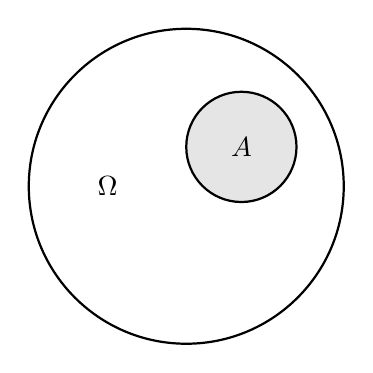
\begin{tikzpicture}[scale=1]
        \draw[thick] (0,0) circle (2cm);
        \node at (-1,0) {$\Omega$};
        \draw[thick, fill=gray!20] (0.7,0.5) circle (0.7cm);
        \node at (0.7,0.5) {$A$};
    \end{tikzpicture}
    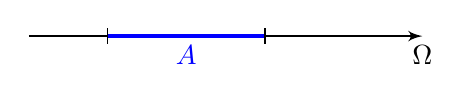
\begin{tikzpicture}[scale=1]
        \draw[thick,->] (0,0) -- (5,0);
        \node[below] at (5,0) {$\Omega$};
        \draw[very thick,blue] (1,0) -- (3,0);
        \node[below,blue] at (2,0) {$A$};
        \draw (1,0.1) -- (1,-0.1);
        \draw (3,0.1) -- (3,-0.1);
    \end{tikzpicture}
    \caption{Continuous random variables}
\end{figure}
Formally, if each event in A is equally likely, then
\begin{equation}
    P[\{x \in A\}] = \frac{\int_{A}dx}{|\Omega|}
\end{equation}
If we relax the assumption of equiprobability, then
more generally
\begin{equation}
    P[\{x\in A\}] = \int_{A} f_X(x) dx
\end{equation}
$f_X(x)$ is called the \emph{probability density function} (PDF).
It is analogous to the probability mass function.

Formally, a probability density function
is a mapping $f_X: \Omega \implies \Re$,
with the following properties:
\begin{itemize}
    \item Non-negativity: $f_X(x) \geq 0 \forall x \in \Omega$
    \item Unity: $\int_{\Omega} f_X(x)dx = 1$
    \item Measure of a set: $P[\{x \in A\}] = \int_{A}f_X(x) dx$
\end{itemize}

We can express a PDF in terms of a PMF
with a train of delta functions like so:
\begin{equation}
    f_X(x) = \sum_{x_k \in \Omega} p_X(x_k) \delta(x - x_k)
\end{equation}

We can also define the probability density
function as the derivative of the CDF, like so:
\begin{equation}
    f_X(x) = \frac{d}{dx}p(X \leq x)
\end{equation}

The expectation of a continuous random variable is
\begin{equation}
    E[X] = \int_{\Omega} xf_X(x)dx
\end{equation}

Properties of the expectation for continuous
random variables:
\begin{itemize}
    \item $E[aX] = aE[X]$
    \item $E[X+a] = E[X] + a$
    \item $E[aX+b] = aE[X] + b$
\end{itemize}

A random variable $X$ has an expectation
if it is absolutely integrable,
\begin{equation}
    E[|X|] = \int_{\Omega} |x|f_X(x)dx < \infty
\end{equation}

The variance of a continuous random variable
$X$ is
\begin{align}
    Var[X] & = E[(X-\mu)^2]                    \\
           & = \int_{\Omega} (x-\mu)^2f_X(x)dx \\
           & = E[X^2] - \mu^2
\end{align}

A continuous \emph{uniform random variable}
has a PDF of
\begin{equation}
    f_X(x) = \begin{cases}
        \frac{1}{b-a} & a \leq x \leq b \\
        0             & \text{else}
    \end{cases}
\end{equation}
We write
\begin{equation}
    X \sim Uniform(a,b)
\end{equation}
to mean that $X$ is drawn from a uniform
distribution on an interval $[a, b]$.
It has a CDF given by
\begin{equation}
    F_X(x) = \begin{cases}
        0               & x < a           \\
        \frac{x-a}{b-a} & a \leq x \leq b \\
        1               & x > b
    \end{cases}
\end{equation}
If $X \sim Uniform(a,b)$ then
\begin{align}
    E[X]   & = \frac{a + b}{2}      \\
    Var[X] & = \frac{(b - a)^2}{12}
\end{align}

A continuous \emph{exponential random variable}
has a PDF of
\begin{equation}
    f_X(x) = \begin{cases}
        \lambda e^{-\lambda x} & x \geq 0    \\
        0                      & \text{else}
    \end{cases}
\end{equation}
\marginnote{An exponential random variable
    is the interarrival time between two consecutive
    Poisson events}
We write
\begin{equation}
    X \sim Exponential(\lambda)
\end{equation}
to mean that $X$ is drawn from an
exponential distribution of parameter
$\lambda$. It has a CDF given by
\begin{equation}
    F_X(x) = 1 - e^{-\lambda x}
\end{equation}
If $X \sim Exponential(\lambda)$, then
\begin{align}
    E[X]   & = \frac{1}{\lambda}   \\
    Var[X] & = \frac{1}{\lambda^2}
\end{align}
Consider $X_n \sim \text{Exponential}(\lambda)$, and let
$X_1, \dots, X_N$ be i.i.d. copies. Define
$Z_N = \sum_{n=1}^{N} X_n$. Then
\begin{equation}
    E[Z_N] = \frac{N}{\lambda}
\end{equation}
and
\begin{equation}
    \text{Var}[Z_N] = \frac{N}{\lambda^2}
\end{equation}


A \emph{Gaussian random variable} is a
random variable $X$ such that its PDF
is
\begin{equation}
    f_X(x) = \frac{1}{\sqrt{2\pi \sigma^2}}\exp\left(-\frac{(x-\mu)^2}{2\sigma^2}\right)
\end{equation}
We write
\begin{equation}
    X \sim Gaussian(\mu, \sigma^2)
\end{equation}
or
\begin{equation}
    X \sim \mathcal{N}\left(\mu, \sigma^2\right)
\end{equation}
to mean that $X$ is drawn from a Gaussian
of parameter $(\mu, \sigma^2)$.
If $X \sim \mathcal{N}(\mu, \sigma^2)$, then
\begin{align}
    E[X]   & = \mu      \\
    Var[X] & = \sigma^2
\end{align}

The \emph{standard Gaussian} random variable has a
PDF given by
\begin{equation}
    f_X(x) = \frac{1}{\sqrt{2\pi}} e^{-\frac{x^2}{2}}
\end{equation}
The CDF of the standard Gaussian is defined
as the $\Phi$ function.
\begin{equation}
    \Phi(x) = \frac{1}{\sqrt{2\pi}}\int_{-\infty}^{\infty} e^{-\frac{t^2}{2}}dt
\end{equation}
The CDF of the standard Gaussian is related to the
\emph{error function}, which is defined as
\begin{equation}
    \text{erf}(x) = \frac{2}{\sqrt{\pi}} \int_{0}^{x} e^{-t^2} dt
\end{equation}
by the relation
\begin{equation}
    \Phi(x) = \frac{1}{2} \left(1 + \text{erf}\left(\frac{x}{\sqrt{2}}\right)\right)
\end{equation}
The CDF of an arbitrary Gaussian is related via
the transformation
\begin{equation}
    F_X(x) = \Phi\left(\frac{x - \mu}{\sigma}\right)
\end{equation}
Let $X \sim \mathcal{N}(\mu, \sigma^2)$, then
\begin{itemize}
    \item $\Phi(y) = 1 -\Phi(-y)$
    \item $P[X\geq b] = 1 - \Phi(\frac{b-\mu}{\sigma})$
    \item $P[|X| \geq b] = 1 - \Phi(\frac{b-\mu}{\sigma}) + \Phi(\frac{-b-\mu}{\sigma})$
\end{itemize}

In addition to mean and variance, we introduce
two more useful quantities, \emph{skewness} and
\emph{kurtosis}.
\begin{align}
    E\left[X\right]                                   & = \mu      \\
    E\left[(X - \mu)^2\right]                         & = \sigma^2 \\
    E\left[\left(\frac{X-\mu}{\sigma}\right)^3\right] & = \gamma   \\
    E\left[\left(\frac{X-\mu}{\sigma}\right)^4\right] & = \kappa
\end{align}
\marginnote{\emph{Excess kurtosis} is defined
    as $\kappa - 3$}

Skewness measures the asymmetry of a
distribution. A Gaussian distribution has
skewness 0. Kurtosis measures how heavy-tailed
the distribution is. If the kurtosis is
positive, then the tails decay faster than a
Gaussian. If the kurtosis is negative, then
the distribution has a tail that
decays more slowly than a Gaussian.

The definition of a CDF is
\begin{equation}
    F_X(x) = P[X \leq x]
\end{equation}
\begin{figure}
    \centering
    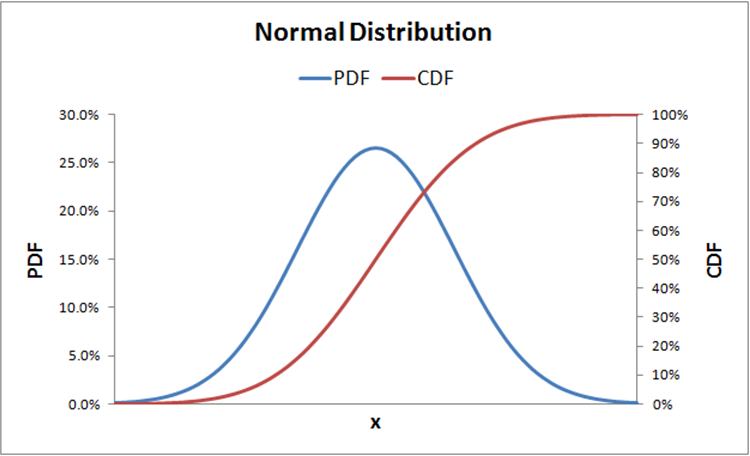
\includegraphics[scale=0.5]{images/normal_distribution_plot.png}
    \caption{PDF and CDF}
\end{figure}
Let $X$ be a continuous random variable. if the CDF
$F_X$ is continuous at any $a\leq x \leq b$, then
\begin{equation}
    P[a \leq X \leq b] = F_X(b) - F_X(a)
\end{equation}
A function $F_X(x)$ is said to be left
continuous if at $x=b$
\begin{equation}
    F_X(b) = \lim_{h\implies 0} F_X(b-h)
\end{equation}
and right continuous if
\begin{equation}
    F_X(b) = \lim_{h\implies 0} F_X(b+h)
\end{equation}
and continuous if $F_X(x)$ is both left
and right continuous.
All CDFs are right continuous.

For any random variable $X$, discrete or continuous,
\begin{equation}
    P[X=b] = \begin{cases}
        F_X(b) - F_X(b^-) & \text{if $F_X$ is discontinuous at $x=b$} \\
        0                 & \text{else}
    \end{cases}
\end{equation}

The PDf is the derivative of the CDF.
\begin{equation}
    f_X(x) = \frac{d}{dx} \int_{-\infty}^{x} f_X(t)dt
\end{equation}
provided $F_X$ is differentiable at $x$. If not, then
\begin{equation}
    f_X(x) = F_X(x) - \lim_{h\implies 0} F_X(x-h)
\end{equation}

Let $X$ be a continuous random variable with PDF
$f_X$. The median of $X$ is a point $c \in \Re$ such that
\begin{equation}
    \int_{-\infty}^{c} f_X(x) dx = \int_{c}^{\infty}f_X(x) dx
\end{equation}

Let $X$ be a continuous random variable. The mode is
the point $c$ such that $f_X(x)$ attains the maximum.
\begin{equation}
    x = \text{argmax}_{x \in \Omega} f_X(x)
\end{equation}

The mean $E[X]$ can be computed from
$F_X$ as
\begin{equation}
    E[X] = \int_{0}^{\infty} (1-F_X(t))dt
\end{equation}

Recall that joint distributions are
higher-dimensional PDFs, PMFs, or CDFs.
\begin{equation}
    f_{\textbf{X}}(\vec{x}) = f_{X_1, \dots, X_N}(x_1, \dots, x_n)
\end{equation}
Let $X$ and $Y$ be two continuous random variables.

The \emph{joint PDF} of $X$ and $Y$ is a function
$f_{X,Y}(x,y)$ that can be integrated to yield a probability
\begin{equation}
    P[A] = \int_{A} f_{X,Y}(x,y)dxdy
\end{equation}
for any event $A \subseteq \Omega_X \times \Omega_Y$.

The \emph{marginal PDF} is defined as
\begin{equation}
    f_X(x) = \int_{\Omega_Y} f_{X,Y}(x,y)dy
\end{equation}
and
\begin{equation}
    f_Y(y) = \int_{\Omega_X} f_{X,Y}(x,y)dx
\end{equation}

The \emph{marginal CDF is}
\begin{align}
    F_X(x) & = F_{X,Y}(x, \infty) \\
    F_Y(y) & = F_{X,Y}(\infty, y)
\end{align}

Let $F_{X,Y}(x,y)$ be the joint CDF of $X$ and $Y$.
Then the joint PDF can be obtained through
\begin{equation}
    f_{X,Y}(x,y) = \frac{\partial^2}{\partial_y\partial_x} F_{X,Y}(x,y)
\end{equation}

If two random variables are \emph{independent},
then
\begin{equation}
    p_{X,Y}(x,y) = p_X(x)p_Y(y)
\end{equation}
and
\begin{equation}
    f_{X,Y}(x,y) = f_X(x)f_Y(y)
\end{equation}

If a sequence of random variables
$X_1, \dots, X_N$ are independent,
then their joint PDF can be factorized.
\begin{equation}
    f_{X_1,\dots,X_N}(x_1,\dots,x_n) = \prod_{n=1}^{N}f_{X_n}(x)n
\end{equation}

A collection of random variables $X_1, \dots, X_N$ are called
\emph{independent and identically distributed} (i.i.d.) if
all are independent and have the same distribution, i.e.
$f_{X_1}(x) = \dots = f_{X_N}(x)$.

The \emph{joint expectation} is
\begin{equation}
    E[XY] = \int_{y\in \Omega_y}\int_{x\in \Omega_x} xy f_{X,Y}(x,y)dxdy
\end{equation}

For an arbitrary $g(X,Y)$,
\begin{equation}
    E[g(X,Y)] = \int_{y\in \Omega_y}\int_{x\in \Omega_x} g(x,y) f_{X,Y}(x,y)dxdy
\end{equation}

Recall
\begin{equation}
    \text{Cov}(X,Y) = E[XY] - E[X]E[Y]
\end{equation}
and now we also state that
\begin{equation}
    \text{Var}[X+Y] = \text{Var}[X] + 2\text{Cov}(X,Y) + \text{Var}[Y]
\end{equation}
We also state that covariance is zero, then so is the correlation.
However if the correlation is zero, the covariance is not necesarily zero.
\begin{equation}
    \text{Cov}(X,Y) = 0 \implies \text{Corr}(X,y) = 0
\end{equation}

If $X$ and $Y$ are independent, then
\begin{equation}
    E[XY] = E[X]E[Y]
\end{equation}
This implies that $X$ and $Y$ are
uncorrelated (i.e. $\text{Cov}(X,Y) = 0$),
but the converse is not true.

Let $X$ and $Y$ be two continuous random variables.
The \emph{conditional PDF} of $X$ given $Y$ is
\begin{equation}
    f_{X|Y}(x|y) = \frac{f_{X,Y}(x,y)}{f_Y(y)}
\end{equation}

Let $X$ and $Y$ be continuous random variables and
$A$ be an event. Then
\begin{equation}
    P[X \in A | Y=y] = \int_{A} f_{X|Y}(x|y)dx
\end{equation}
\begin{equation}
    P[X\in A] = \int_{\Omega_Y} P[X\in A|Y = y]f_Y(y)dy
\end{equation}

The \emph{conditional expectation} of $X$ given $Y=y$ is
\begin{equation}
    E[X|Y=y] = \int_{-\infty}^{\infty}xf_{X|Y}(x|y)dx
\end{equation}

The \emph{law of total expectation} is
\begin{equation}
    E[X] = \int_{-\infty}^{\infty} E[X|Y=y]f_Y(y)dy
\end{equation}
The theorem is sometimes also written
\begin{equation}
    E[X] = E_Y[E_{X|Y}[X|Y]]
\end{equation}

\appendix

\section{Reference}
\setcounter{equation}{0}


\subsection{Series}
\begin{equation}
    \sum_{k=0}^{n} r^k = \frac{1 - r^{n + 1}}{1 - r}
\end{equation}
\begin{equation}
    \sum_{n=1}^{\infty} \frac{1}{n^2} = \frac{\pi^2}{6}
\end{equation}
\begin{equation}
    \sum_{k=1}^{\infty}kr^{k - 1} = \frac{1}{(1 - r)^2}
\end{equation}

\subsection{Combinatorics}
\begin{equation}
    {n\choose k} = \frac{n!}{k!(n - k)!}
\end{equation}
\begin{equation}
    (a + b)^n = \sum_{k=0}^{n} {n\choose k} a^{n - k}b^k
\end{equation}
\begin{equation}
    {n\choose k} + {n\choose k-1} = {n + 1\choose k}
\end{equation}
\begin{equation}
    P(n, k) = \frac{n!}{(n-k)!}
\end{equation}
where $P(n, k)$ is the number of ways to arrange $k$ objects out of $n$ (permutations).
\begin{equation}
    C(n, k) = {n\choose k} = \frac{n!}{k!(n-k)!}
\end{equation}
where $C(n, k)$ is the number of ways to choose $k$ objects out of $n$ (combinations).

\subsection{Approximations}
\begin{align}
    f(x) & = f(a) + f'(a)(x - a) + \frac{f''(a)}{2!}(x - a)^2 + \dots \\
         & = \sum_{n=0}^{\infty} \frac{f^{(n)}(a)}{n!}(x - a)^n
\end{align}
\begin{align}
    1 + x + \frac{x^2}{2!} + \frac{x^3}{3!} + \dots & = \sum_{k=0}^{\infty} \frac{x^k}{k!} \\
                                                    & = e^x
\end{align}
\begin{align}
    \sin(x) & = x - \frac{x^3}{3!} + \frac{x^5}{5!} - \frac{x^7}{7!} + \dots \\
            & = \sum_{n=0}^{\infty} (-1)^n \frac{x^{2n+1}}{(2n+1)!}
\end{align}
\begin{align}
    \cos(x) & = 1 - \frac{x^2}{2!} + \frac{x^4}{4!} - \frac{x^6}{6!} + \dots \\
            & = \sum_{n=0}^{\infty} (-1)^n \frac{x^{2n}}{(2n)!}
\end{align}
\begin{align}
    \ln(1 + x) & = x - \frac{x^2}{2} + \frac{x^3}{3} - \frac{x^4}{4} + \dots \\
               & = \sum_{n=1}^{\infty} (-1)^{n+1} \frac{x^n}{n}
\end{align}

\subsection{Calculus}
\begin{equation}
    \frac{d}{dx} \int_{a}^{x} f(t)\,dt = f(x)
\end{equation}
\begin{equation}
    \int_{a}^{b} f'(x)\,dx = f(b) - f(a)
\end{equation}
\begin{equation}
    \int f(g(x))g'(x)\,dx = \int f(u)\,du
\end{equation}
\begin{equation}
    \int u\,dv = uv - \int v\,du
\end{equation}
\begin{equation}
    \int \frac{1}{(x-a)(x-b)}\,dx = \frac{1}{b-a} \ln\left|\frac{x-a}{x-b}\right| + C
\end{equation}

\subsection{Linear Algebra}
\begin{equation}
    \vec{y} = \beta_1 \vec{x_1} + \beta_2 \vec{x_2} + \cdots + \beta_N \vec{x_N}
\end{equation}
\begin{align}
    \langle \vec{a}, \vec{b} \rangle & = \vec{a}\vec{b}^{T}     \\
                                     & = \sum_{i=1}^{n} a_i b_i
\end{align}
where $\langle \vec{a}, \vec{b} \rangle$ denotes the inner product of vectors $\vec{a}$ and $\vec{b}$.
\begin{equation}
    \|\vec{x}\|_p = \left( \sum_{i=1}^{n} |x_i|^p \right)^{1/p}
\end{equation}
where $\|\vec{x}\|_p$ is the $p$-norm (or $\ell_p$-norm) of vector $\vec{x}$.
\begin{equation}
    \cos(\theta) = \frac{\langle \vec{a}, \vec{b} \rangle}{\|\vec{a}\|_2 \|\vec{b}\|_2}
\end{equation}
where $\theta$ is the angle between vectors $\vec{a}$ and $\vec{b}$.
\begin{equation}
    \hat{\beta} = (\mathbf{X}^T \mathbf{X})^{-1} \mathbf{X}^T \vec{y}
\end{equation}
where $\hat{\beta}$ is the vector of least squares coefficients, $\mathbf{X}$ is the data matrix, and $\vec{y}$ is the target vector

\end{document}